% contenu du fichier : chap1.tex
%
\chapter{Notions et préliminaire}
Dans le présent chapitre, nous présentons l'importance de notre domaine de recherche de façon très générale puis on introduit des termes et des concepts qui seront utilisés tout au long de cette thèse: réseaux complexe, théorie des graphes, distribution des degrés, etc.
 \section{Les réseaux complexes}
  \subsection{Définition}
  Un \textsf{réseau} est tous simplement une collection de points réunis sous forme de paires, les points sont appelés nœuds ou sommets et les lignes sont appelées liens ou bords. Le mots \textsf{complexe} est en général le résultat de  l'évolution décentralisée et non planifiée dans ces réseaux (Fig.~\ref{exemples-reseaux}). De nombreux objets d'intérêt dans les sciences physiques, biologiques et sociales peuvent être considérés comme des réseaux complexes, cette nouvelle façons de penser conduit souvent à de nouvelles et utiles idées. Alors un réseau est une représentation simplifiée qui réduit un système à une structure abstraite capturant uniquement les bases des modèles de connexion, les nœuds et les liens d'un réseau peuvent être accompagnés d' informations supplémentaires pour capturer plus de détails sur le système, même s'il y a un inconvénient de perte d'informations dans le processus de réduction d'un système complet à une représentation par réseau, mais il présente également des grands avantages.
  
  \begin{figure}[h!]
  	\centering
  	\includegraphics[scale=0.95]{./figures/exemples-reseaux}
  	\caption{Représentation de quelques types de réseaux composés par des nœuds et des arêtes. }
  	\label{exemples-reseaux}
  \end{figure}
  \subsection{Différents types des Réseaux complexes}
  L'étude des réseaux complexes a été inspirée par le désir de comprendre les différents systèmes réels, allant des réseaux de communications aux réseaux écologiques. Les bases de données empiriques disponibles pour l'étude couvrent plusieurs disciplines, en générale, elles se divisent en quatre grandes catégories: Réseaux Technologique, Réseaux Biologiques, Réseaux Sociaux
  et Réseaux d'Informations.
  \subsubsection{Réseaux Technologique}
  Les réseaux technologiques sont des réseaux artificiels, qui ont grandi au cours du siècle dernier et qui constituent une grande partie de notre société moderne, comme les réseaux électriques, réseaux téléphoniques, réseaux de transports, etc \cite{Pi1965,Am-al2000,Do-al2007,Se-al2003}.
  L'Internet est parmi les exemples les plus connus et les plus largement étudiés des réseaux technologiques (voir Fig.~\ref{Internet}), on peut le définir comme un réseau de données informatiques dans lequel les nœuds sont des ordinateurs et les liens sont des connexions de données physiques entre eux, tels que des câbles à fibres optiques ou des lignes téléphoniques \cite{F-al1999,BC2001}. Il est curieux que, bien que l'Internet est un réseau artificiel, nous ne connaissons pas exactement sa structure, nos meilleures données actuelles sur sa structure proviennent d'études expérimentales.
  \begin{figure}[h!]
  	\centering
  	\includegraphics[width=11cm,height=6cm]{./figures/Internet3}
  	\caption{Nous avons ici un affichage hyperbolique de blogs en utilisant à la fois les ensembles de données WWE et ICWSM 2007 (http://datamining.typepad.com/).}
  	\label{Internet}
  \end{figure}

  Il existe un certain nombre d'excellentes raisons pratiques pour être intéressé à étudier la structure du réseau d'Internet, la fonction d'Internet consiste à transporter des données entre ordinateurs dans différentes parties du monde, ce qui se fait en divisant les données en pièces ou en paquets et en les transportant d'un nœud à l'autre sur le réseau jusqu'à ce 
  qu'ils atteignent leur destination, sans aucun doute, la structure du réseau affectera la manière dont il accomplit efficacement cette fonction et si nous connaissons la structure du réseau, nous pouvons aborder de nombreuses questions et problèmes de pertinence pratique.
  
  
  \subsubsection{Réseaux Biologiques}
  Une autre classe des  réseaux les plus étudiées dans la littérature est celle des réseaux biologiques. Cette classe contient une grande variété de réseaux naturels. Le corps, qu'il soit humain ou animal, contient un grand nombre de réseaux, dont certains se produisent dans l'espace réel, tels que le système nerveux. Ces réseaux ont été étudiés depuis longtemps \cite{WB1997}.
  Une autre classe de réseau, ce sont les réseaux d'interactions gène-gène, protéines-gène et protéines-protéines \cite{DM2003}, ainsi que les réseaux d'interactions entre les espèces dans les écosystèmes, comme la prédation ou la coopération.\\
\begin{figure}[h!]
\centering
\includegraphics[scale=0.2]{./figures/PPI}
\caption{Un réseau modulaire est illustré au moyen du protéome humain (données obtenues à partir de la base de données DIP: http://dip-doe-mbi.ucla.edu). Les nœuds sont des protéines et des liens indiquent leur interaction physique (protéine-protéine).}
\label{PPI}
\end{figure}
 La structure de ces réseaux se diffère selon chaque cas. Par exemple, les réseaux métaboliques sont des réseaux de protéines interagissant les uns avec les autres à l'intérieur de la cellule Fig.~\ref{PPI}, il s'agit d'un réseau dirigé, car chaque protéine peut catalyser ou réprimer la création d'autres protéines, ce qui n'implique pas nécessairement le processus inverse. La structure à grande échelle des réseaux métaboliques a été étudiée pour de nombreuses espèces, il a été trouvé que ces réseaux ont une distribution des degrés sans-échelle \cite{Je-al2000}. De plus, il a été observé que le diamètre du réseau est très petit et presque indépendant de la taille du réseau, cette indépendance s'explique par que certain classe de réseaux sans-échelle est Ultra-small \cite{Cohen-Havlin2003,Do-al2003,ChL2003}, d'une autre coté notre résultats du troisième chapitre renforcent cette explication et indiquent que la dépendance du diamètre avec la taille $N$ est très faible.\\ Dans les réseaux génétiques, les nœuds représentent des gènes, et les liens sont dirigés  et représentent l'influence d'un gène sur un autre, le réseau E. coli est un des réseaux génétiques qui est bien étudiés dans la littérature \cite{Mi-al2002}.


  \subsubsection{Réseaux Sociales}
  Un réseau social est un ensemble de nœuds, où ces nœuds se représente par des  personnes  (individus ou groupes sociaux) et les liens par une relation qui peut être de parenté, amitié, statut, etc \cite{JS2000}, cette diversité des liens est une chose appréciée dans l'étude des réseaux sociaux, car il existe de nombreuses définitions possibles d'un tel réseau et la définition particulière que l'on utilisera dépendra des questions auxquelles on est intéressé à répondre. Tel que les réseaux d'amitiés entre les individus \cite{WW1977,Mo1934}, les relations d'affaires entre les entreprises \cite{JP1977}.
  La société offre une grande variété d'organisations de groupes possibles: les familles, les milieux de travail et d'amitié, les villages, les villes, les nations. La diffusion d'Internet a également conduit à la création de groupes virtuels, en direct sur le Web, comme Facebook qui reliant presque tout  notre monde entier (voir Fig.~\ref{Facebook}).
  
\begin{figure}[h!]
\centering
\includegraphics[width=9cm,height=5cm]{./figures/facebook}
\caption{Le 'Social Graph' derrière Facebook, graphe des relation d'amis de $500$ million personnes, image par Paul Butley, $2010$.}
\label{Facebook}
\end{figure}
Bien avant que l'Internet commence à jouer un rôle important dans la vie de beaucoup de personnes, les sociologues et d'autres chercheurs des sciences humaines ont examiné la structure des groupes de personnes. Dans la plupart des cas, des groupes relativement petits ont été considérés, nécessairement parce que l'analyse de grands groupes n'était pas souvent possible.\\
Une contribution importante à l'analyse des réseaux sociaux est venue de Jacob Moreno qui a introduit des sociogrammes dans les années 1930. Un sociogramme peut être considéré comme une représentation graphique d'un réseau: les personnes sont représentées par des points (appelés nœuds) et leurs relations par des lignes reliant ces points (appelés arêtes).\\
L'analyse des réseaux sociaux a été importante pour le développement ultérieur de la théorie des graphes, par exemple en ce qui concerne l'introduction de mesures pour identifier l'importance des personnes ou des groupes. Par exemple, une personne ayant de nombreuses connexions avec d'autres personnes peut être considérée comme relativement importante. De même, une personne au centre d'un réseau semble être plus influente que quelqu'un au bord. Ce que la théorie des graphes nous fournit, ce sont les outils pour décrire formellement l'importance et l'influence des nœuds. En outre, en utilisant la théorie des graphes, nous pouvons facilement proposer des solutions alternatives pour décrire l'importance des personnes. L'existence de ces outils a également améliorer la précision des déclarations concernant le poste ou le rôle de ces personnes au sein d'une communauté.
  \subsubsection{Réseaux d'informations}        
 Les  réseaux de citation et le World Wide Web (WWW), comme dans Fig.~\ref{WWW}, sont un bon exemple des réseaux d'informations, car leur contenu d'informations étant stockée dans des nœuds, c’est pour cette raison que l’on utilise le terme réseau d’informations. Parfois on rencontre une certaine confusion à propos de réseau  WWW  et le réseau d'Internet. Dans la WWW, les nœuds sont les pages HTML, et les bords représentent les liens entre les pages, par contre  dans l'Internet, les liens correspondent aux câbles physiques entre les ordinateurs. Alors  le WWW est virtuelle et Internet est physique.
\begin{figure}[h!]
	\centering
	\includegraphics[scale=0.3]{./figures/www2}
	\caption{La structure de l'Internet au niveau des systèmes autonomes. Les nœuds de cette représentation sont des systèmes autonomes et les bords montrent les itinéraires empruntés par les données qui circulent entre eux. La photo a été créée par Hal Burch et Bill Cheswick en 2009.}
	\label{WWW}
\end{figure}

\section{Les réseaux complexes, la physique moderne et l'unification}
La physique explique les phénomènes de la nature en les réduisant à une interaction de lois fondamentales simples. Cette méthode plutôt réussie semble rencontrer certaines difficultés lorsqu'il s'agit des systèmes complexes en général et des réseaux complexes en particulier. Dans ces derniers il reste peu clair s'il existe des lois universelles uniques expliquant une variété de similitudes structurelles et dynamiques trouvées dans de nombreux réseaux réels différents  \cite{K-al2012,BS2009,La-al2009,Li-al2011}. En revanche, l'\textsf{unification} des lois universelles qui paraissaient jusqu'alors complètement séparées sont-elles d'une  origine commune ? c'est ce que les physiciens théoriques rêvent de découvrir. Une telle  \textsf{unification}
va \^{e}tre, sans doute, un grand pas dans notre compréhension de la nature. En outre, l'existence de cette belle idée au cœur de l'unification montre le pouvoir mystérieux que les êtres humains peuvent découvrir derrière les apparences de la nature \cite{Sm1997}.

Le réseau causal représentant la structure à grande échelle de l'espace-temps dans notre univers accéléré est un graphe de loi de puissance avec un regroupement fort, similaire à de nombreux réseaux complexes tels que les réseaux Internet, sociaux ou biologiques \cite{K-al2012}. Cette similitude structurelle est une conséquence de l'équivalence asymptotique entre la dynamique
de croissance à grande échelle des réseaux complexes et des réseaux causaux. Par conséquent, un intérêt croissant est adressé à l'étude de la gravité quantique à partir de la théorie de l'information et de la perspective des réseaux complexes \cite{Tr2015,Bi-al2015}.

Récemment, des relations intrigantes entre les propriétés des réseaux de communication quantique avec des topologies de réseau et la physique statistique ont été rapportées. Sur la base des concepts classiques de percolation \cite{BR2006}, il a été montré que ces réseaux quantiques peuvent présenter une transition de phase de percolation d'enchevêtrement \cite{Ac-al2007,Sa1999}.
L'avancement rapide de la technologie de l'information quantique a suscité un intérêt considérable pour les propriétés dynamiques des réseaux quantiques formés par les systèmes élémentaires, tels que les qubits, en raison de leur rôle privilégié dans la communication et le calcul quantiques \cite{J-al2015,BG2007,MC2000}.\\

Une autre domaine de recherche en relation avec les sciences des réseaux et notamment aux réseaux complexes. La science générale des réseaux et de ses diverses applications a une pertinence significative pour les praticiens de l'intelligence artificiel (IA). Par exemple, la compréhension de la structure d'Internet et du World Wide Web sera importante pour l'orientation de la direction de l'intelligent, l'équilibrage de charge, la recherche de toutes sortes et le déploiement d'agents\footnote{Un agent est un terme important en IA qui désigne une entité capable d’interagir avec
	son environnement.} intelligents qui assistent les utilisateurs dans leurs tâches réseau. La réflexion en réseau sera également fondamentale pour développer des algorithmes décentralisés efficaces pour les réseaux de calcul, de communication et de détection de plus en plus distribués et liés, ainsi que des méthodes de sécurité efficaces pour ces systèmes de plus en plus vulnérables. Ce sont tous des domaines dans lesquels la recherche sur l'IA et l'apprentissage automatique ont joué et joueront un rôle majeur \cite{Mitchell2006,Basheer-Hajmeerb2000,Passerini-al2017}.

\section{La théorie des graphes}
En terme générale, un réseau se décrit comme un graphique dont les nœuds (sommets) identifient les éléments du
système et les liens de connexion (arêtes) représente la présence d'une relation ou d'une interaction entre ces
éléments. Avec un tel niveau de généralité, il est facile de percevoir qu'un large éventail de systèmes peuvent être abordés
dans le cadre de la théorie du graphe. Alors nous fournissons ici un bref historique et quelques notations de base nécessaires
dans la théorie de graphe pour décrire les réseaux. Le cadre naturel pour une description mathématique rigoureuse des réseaux
se trouve dans la théorie des graphes, mais il faut noter que la théorie des graphes 
constitue une branche des mathématiques vaste et compliquée et nous ne sommes pas dans l'état de fournir une présentation formelle et complète de 
celle-ci. Cependant notre but dans ce chapitre d'introduction est de fournir seulement quelques notions utiles pour décrire 
les réseaux dans la suite de cette thèse. Pour les lecteurs souhaitant aller plus en détail dans l'étude de la théorie des graphes pourraient consulter ces livres \cite{Ha1995,West1996}.
  \subsection{Bref historique}
  En plus de la topologie, Euler est devenue le père de la théorie des graphes quand il a résolu, en $1736$, un problème célèbre
sous le nom \textit{"le problème du pont de K\"{o}nigsberg"}, la question était de savoir s'il était possible de visiter les quatre
quartiers de la ville séparés les uns des autres par un bras de rivière, en passant exactement une fois par chaque pont et en 
revenant à son point de départ (voir Fig.~\ref{Konig}).
\begin{figure}[h!]
\centering
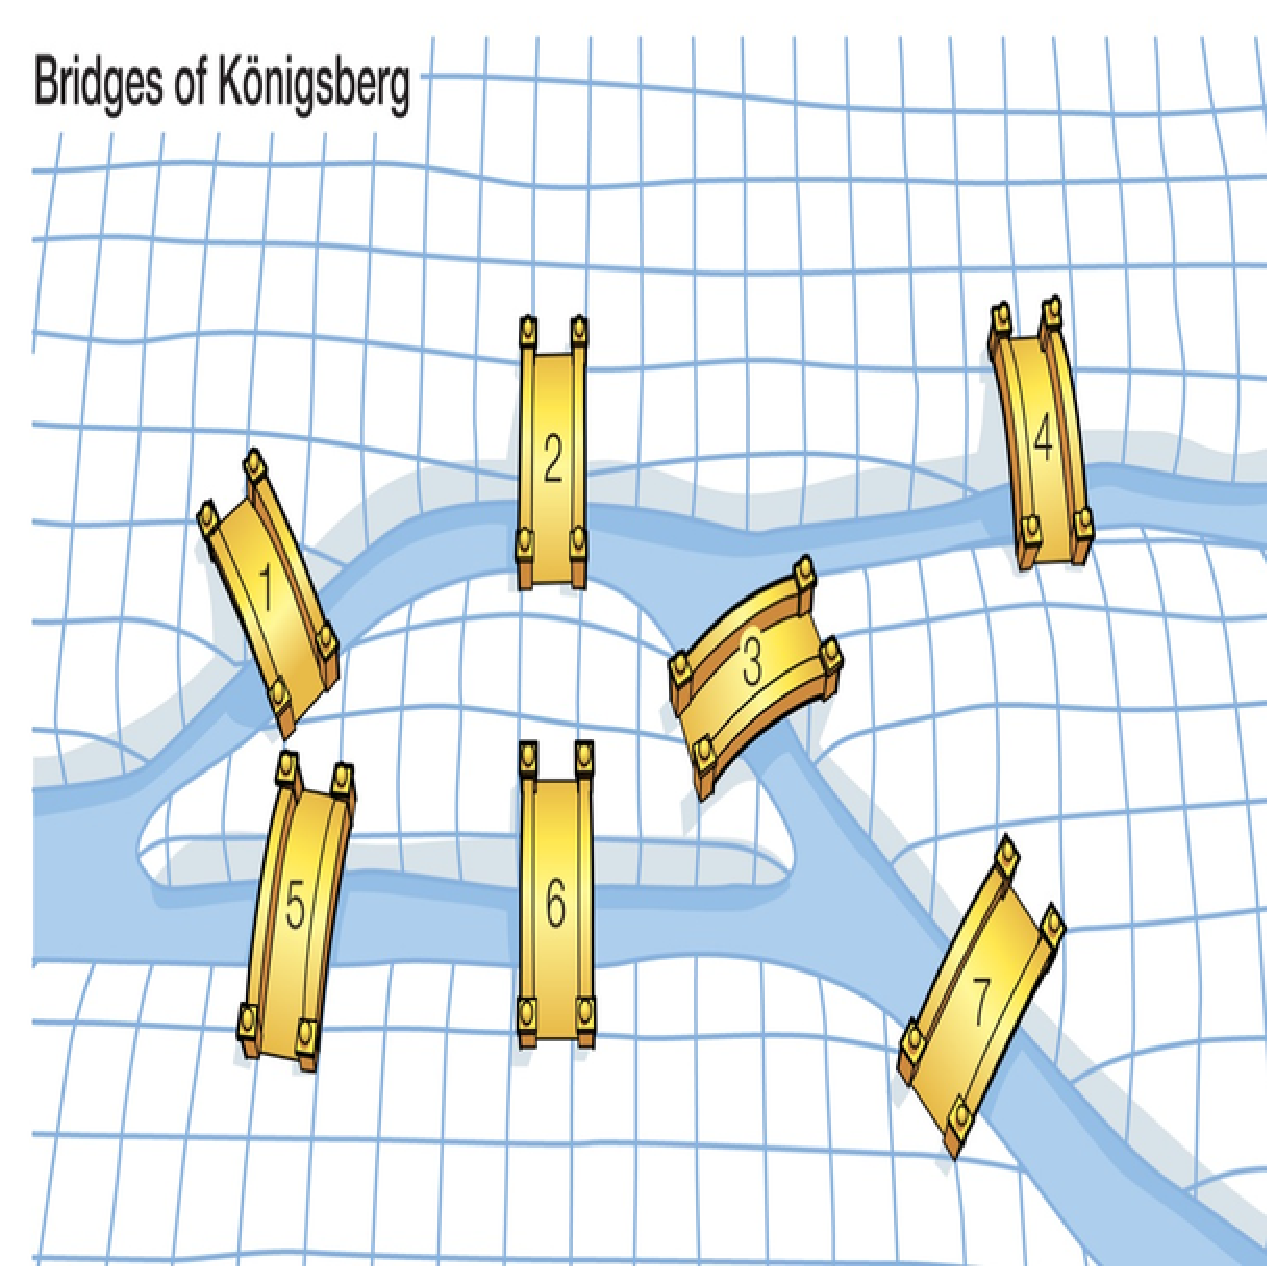
\includegraphics[scale=0.7]{./figures/Konig}
\caption{Ponts de K$\ddot{o}$nigsberg, $1736$}
\label{Konig}
\end{figure}
Afin de trouver une solution à ce problème Euler a remplacé chaque zone de terrain par un point et chaque pont par une ligne 
joignant les points correspondants, produisant ainsi un \textit{"graphe"}. Ainsi il a montré que le problème
est insoluble et que le graphe de cette ville ne peut pas être parcouru d'une certaine manière.

En $1847$ Kirchhoff a développé la théorie des arbres afin de résoudre le système d'équations linéaires simultanées qui 
donnent le courant dans chaque branche et autour de chaque circuit d'un réseau électrique. Bien qu'un physicien, il a pensé comme un mathématicien lorsqu'il a remplacé un réseau électrique par sa structure combinatoire  correspondante constituée uniquement de points et de lignes sans indication du type d'élément électrique représenté par des lignes individuelles.
Dans les années $1960$, deux mathématiciens, Paul Erd\H{o}s et Alfred Rényi (ER), ont introduit une nouvelle idée ingénieuse, ils ont 
combiné les concepts de la théorie graphique avec les outils de la théorie des probabilités, cela permettant d'envisager des
familles de graphes plutôt que des graphes spécifiques.

  \subsection{L’expérience de Milgram}
 \label{Milgram} 
En $1967$, Stanley Milgram a effectué une expérience intéressante.  Dans sa première expérience, Milgram a demandé à des personnes choisies au hasard au Nebraska d'envoyer des lettres à une personne cible éloignée à Boston.
Les participants ne pouvaient passer que les lettres (à la main) aux connaissances personnelles qu'ils pensaient pouvoir 
atteindre la cible, soit directement, soit via un % «ami d'un ami».  dans sa première experience seules trois lettres ont
finalement atteint leur destination. Mais dans les expériences ultérieures, Milgram a réussi à augmenter
le taux de réussite à $95\%$, pour plus de détails (voir \cite{Mi1967,TM1969}). La conclusion principale du cette expérience
de Milgram était que la plupart des gens sur notre planète n'est séparé que par six autres personnes en moyen. Cette idée de
Milgram a été reprise encore une fois en 2001 par Duncan Watts et ses collègues en utilisant un message électronique qui devait être livré à des expéditeurs autour de monde, étonnamment, Watts a constaté que le nombre moyen d'intermédiaires était
$6$. Pour plus de détails et une analyse statistique beaucoup plus étendue des données par rapport à l'analyse de Milgram,
voir Dodds et al \cite{D-al2003}.

  \subsection{Représentation d'un graphe}
  Comme dans toute abstraction mathématique, lorsque nous décrivons un système en tant que graphe, nous décidons de rejeter  plusieurs des particularités particulières des phénomènes réels et de nous concentrer uniquement sur quelques caractéristiques  d'intérêt. En particulier, un graphe est essentiellement un moyen de coder une relation, liens physiques, interactions,
  etc, entre les éléments d'un système. Les éléments du système identifient l'ensemble $V$ (ensemble des nœuds) et les relations entre ceux de l'ensemble $E$ (ensemble des arêtes). Le graphe indiqué comme $G(V, E)$ peut être présenté en traçant les  nœuds en tant que points et les bords comme lignes entre eux.\\ 
 
   Parmi les façons de présentation basées sur cette définition on peut citer la matrice d'adjacence et la liste adjacence:
  \subsubsection{La matrice d’adjacence}
 Un graphe est représenté fréquemment par une matrice d'adjacence, $M_{i,j}$, dans laquelle chaque ligne et
 chaque colonne représente un nœud du graphe. Dans un graphe non-dirigé l'élément $M_{i,j}=1$ si un lien existe entre le $i^{eme}$ et $j^{eme}$
 nœud sinon $M_{i,j}=0$  (voir Fig.~\ref{matrice d'adjacence}), ainsi la matrice sera en général asymétrique et les éléments diagonaux ne sont pas
 nécessairement $0$.
  \begin{figure}[h]
 	\centering
 	\subfloat{
 		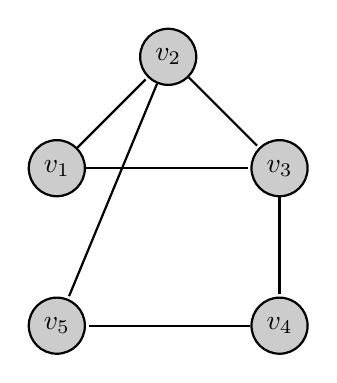
\begin{tikzpicture}[shorten >=1pt,auto,node distance=2cm,thick,main node/.style={circle,fill=black!20,draw}]
 		%[-,>=stealth',shorten >=1pt,auto,node distance=2cm,thick,main node/.style={circle,fill=black!20,draw}]
 		\node[main node] (1) {$v_2$};
 		\node[main node] (2) [below left of=1] {$v_1$};
 		\node[main node] (3) [below right of=1] {$v_3$};
 		\node[main node] (4) [below of=3] {$v_4$};
 		\node[main node] (5) [below of=2] {$v_5$};
 		
 		\path[every node/.style={font=\sffamily\small}]
 		(2) edge node [left] {} (1)
 		(2) edge node [left] {} (3)
 		(1) edge node [left] {} (5)
 		(1) edge node [left] {} (3)
 		(3) edge node [left] {} (4)
 		(4) edge node [left] {} (5)
 		;
 		\end{tikzpicture}}
 	\subfloat{
 		\vbox{\hbox{
 				\begin{math}
 				M_{G} = \left(
 				\begin{array}{ccccc}
 				0 & 1 & 1 & 0 & 0 \\
 				1 & 0 & 1 & 0 & 1 \\
 				1 & 1 & 0 & 1 & 0 \\
 				0 & 0 & 1 & 0 & 1 \\
 				0 & 1 & 0 & 1 & 0
 				\end{array}
 				\right)
 				\end{math}
 			}% end of first hbox
 			\null% last null hbox, which sets the baseline of the \vbox
 		} % end of vbox
 	} % end of subfloat
 	\caption{Exemple d'un graphe non-orienté et sa matrice d'adjacence $M_G$ avec 5 nœuds et 6 arêtes.}
 	\label{matrice d'adjacence}
 \end{figure}  
 
  Un graphe orienté est un graphe où les bords sont dirigés, c'est-à-dire que chaque bord est une paire de nœuds ordonnée avec ($i$,$j$) désignant un bord (flèche) qui commence au nœud $i$ et se termine au nœud $j$ Fig.~\ref{matrice d'adjacence2}. 
 
 
 \begin{figure}[h]
	\centering
	\subfloat{
		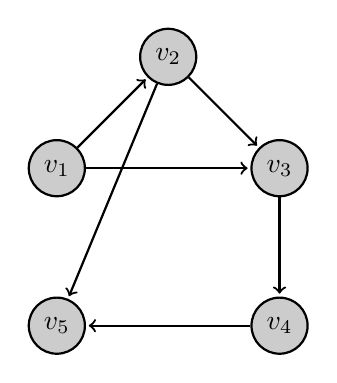
\begin{tikzpicture}[->,shorten >=1pt,auto,node distance=2cm,thick,main node/.style={circle,fill=black!20,draw}]
		%[-,>=stealth',shorten >=1pt,auto,node distance=2cm,thick,main node/.style={circle,fill=black!20,draw}]
		\node[main node] (1) {$v_2$};
		\node[main node] (2) [below left of=1] {$v_1$};
		\node[main node] (3) [below right of=1] {$v_3$};
		\node[main node] (4) [below of=3] {$v_4$};
		\node[main node] (5) [below of=2] {$v_5$};
		
		\path[every node/.style={font=\sffamily\small}]
		(2) edge node [left] {} (1)
		(2) edge node [left] {} (3)
		(1) edge node [left] {} (5)
		(1) edge node [left] {} (3)
		(3) edge node [left] {} (4)
		(4) edge node [left] {} (5)
		;
		\end{tikzpicture}}
	\subfloat{
		\vbox{\hbox{
				\begin{math}
				M_{G} = \left(
				\begin{array}{ccccc}
				0 & 0 & 0 & 0 & 0 \\
				1 & 0 & 0 & 0 & 0 \\
				1 & 1 & 0 & 0 & 0 \\
				0 & 0 & 1 & 0 & 0 \\
				0 & 1 & 0 & 1 & 0
				\end{array}
				\right)
				\end{math}
			}% end of first hbox
			\null% last null hbox, which sets the baseline of the \vbox
		} % end of vbox
	} % end of subfloat
	\caption{Exemple d'un graphe orienté et sa matrice d'adjacence $M_G$ avec 5 nœuds et 6 arêtes.}
	\label{matrice d'adjacence2}
\end{figure}


\subsubsection{La liste d’adjacence}
Le format de liste d'adjacence est utile pour les graphes sans données associées aux nœuds ni aux bords et à des nœuds
qui peuvent être représentés de manière significative sous la forme de chaînes, il se compose de 
lignes avec des étiquettes de nœud, la première étiquette dans une ligne est le nœud source, les autres étiquettes dans la
ligne sont considérées comme des nœuds cibles et sont ajoutées au graphe avec un bord entre le nœud source et le nœud 
cible.\\
\begin{figure}[h]
	\centering
	\subfloat{
		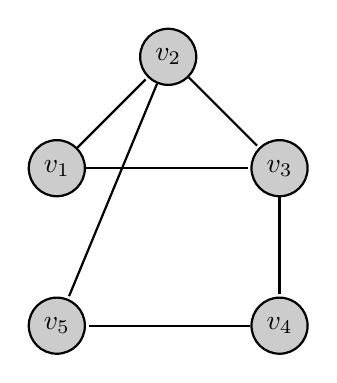
\begin{tikzpicture}[shorten >=1pt,auto,node distance=2cm,thick,main node/.style={circle,fill=black!20,draw}]
		%[-,>=stealth',shorten >=1pt,auto,node distance=2cm,thick,main node/.style={circle,fill=black!20,draw}]
		\node[main node] (1) {$v_2$};
		\node[main node] (2) [below left of=1] {$v_1$};
		\node[main node] (3) [below right of=1] {$v_3$};
		\node[main node] (4) [below of=3] {$v_4$};
		\node[main node] (5) [below of=2] {$v_5$};
		
		\path[every node/.style={font=\sffamily\small}]
		(2) edge node [left] {} (1)
		(2) edge node [left] {} (3)
		(1) edge node [left] {} (5)
		(1) edge node [left] {} (3)
		(3) edge node [left] {} (4)
		(4) edge node [left] {} (5)
		;
		\end{tikzpicture}}
	\subfloat{
		\vbox{\hbox{
				\begin{math}
				\begin{tabular*}{0.5\textwidth}{@{\extracolsep{\fill}}ccc} \toprule Noueds	& voisins\\ \midrule 1	& 2,3\\ 2	& 1,3\\ 3	& 1,2,4\\ 4	& 3,5\\ 5 & 2,4 \\ \bottomrule
				\end{tabular*}			
				\end{math}
			}% end of first hbox
			\null% last null hbox, which sets the baseline of the \vbox
		} % end of vbox
	} % end of subfloat
	\caption{Exemple d'un graphe non-orienté et sa liste d'adjacence avec 5 nœuds et 6 arêtes.}
	\label{matrice d'adjacence1}
\end{figure}

En règle générale, les matrices sont utilisées pour les tableaux denses et les listes d'adjacence pour les 
tableaux dispersés. La raison est que les matrices consomment moins d'espace pour les tableaux denses et les listes
d'adjacence consomment moins d'espace pour les tableaux dispersés. Cependant, l'espace n'est qu'une considération, d'autres
facteurs doivent également être pris en compte.


\section{Caractéristiques des réseaux complexes}

On croit que ne comprend pas encore les réseaux de manière appropriée. Par exemple, si les données (la matrice d'adjacence) d'un grand graphe sont présentes et que vous n'êtes pas autorisé à visualiser le réseau,
il semble assez complexe de dire simplement quelles sont les propriétés du réseau. Alors
l'étude de ces réseaux oblige à ajouter d'autres caractéristiques supplémentaires, telles que, le plus court chemin,
Clustering, etc.
   \subsection{Plus court chemin}
   
   Le plus court chemin entre deux nœuds d'un graphe est défini comme étant la longueur du trajet le plus court parmi tous les trajets possibles. Une
   mesure statistique globale de la distance entre les nœuds peut alors être exprimée comme la valeur moyenne des chemins les
   plus courts entre tous les couples possibles de nœuds du réseau, mathématiquement on peut le définir par la forme suivante
   \begin{equation}
    l=\frac{1}{n(n-1)}\sum_{i,j} d_{i,j},
   \end{equation}
   avec $d_{ij}$ est la distance la plus courte du nœud $i$ au nœud $j$ et $n$ est le nombre total de nœuds dans le réseau. Sachant que la distance entre deux nœuds qui ne sont pas atteignables de l'un à l'autre est $0$  et la distance d'un nœud à lui-même est également $0$.\\
   Dans de nombreux réseaux à grande échelle, la distance moyenne entre les nœuds est très faible par rapport à la taille du graphe, ce phénomène est connu sous le nom de la propriété \textit{petit-monde}. Cette propriété a été popularisé dans le contexte sociologique où elle est parfois appelée \textit{six degrés de séparation}\cite{Mi1967}.\\
   L'importance de cette propriété consiste en son rôle important dans le transport et la communication au sein d'un réseau. Supposons qu'il soit nécessaire d'envoyer un paquet de données d'un ordinateur à un autre via Internet: la géodésique fournit un chemin  optimal, car on pourrait obtenir un transfert rapide et conserver les ressources du système \cite{PV2004}. Pour une telle raison, les chemins les plus courts ont également joué un rôle important dans la caractérisation de la structure interne d'un graphe \cite{Wa1994,JS2000,Bo-al2006}.

   Les ensembles de données massifs du réseau s'accumulent à un rythme énorme dans des champs variés \cite{Qi-al2010}. En utilisant la mesure moyenne du plus court chemin, les réseaux de petit-monde peuvent être considérés comme des systèmes à la fois efficaces à l'échelle mondiale et locale \cite{Latora-Marchiori2001}. Nous utilisons souvent la longueur du plus court chemin comme mesure de l'efficacité du réseau, ce qui nous permet de donner une analyse quantitative précise de l'efficacité du flux d'information dans les réseaux. Le calcul du plus court chemin a également été utilisé pour estimer la précision des approximations analytiques de la dynamique sur les réseaux \cite{Melnik-al2011}, en examinant l'apparition de la synchronisation \cite{Zhao-al2006} et en évaluant la résilience des réseaux de communication aux attaques et aux échecs \cite{Albert-al2000}.
   
   \subsection{Coefficient de regroupement (Clustering)}
   En plus de l'effet du petit-monde un haut niveau de regroupement s'en accompagne dans de nombreux
   réseaux sociaux et différents autres réseaux ont montré cette tendance également, notamment le réseau mondial \cite{Lad1999}, les réseaux de transport \cite{Seb-al2022} et les réseaux métaboliques \cite{WD2000,SC2001}.
   Le concept de regroupement d'un graphe
   se réfère à la tendance observée dans de nombreux réseaux naturels à former des cliques au voisinage d'un nœud donné, 
   cette propriété est appelée également la transitivité dans le contexte de la sociologie \cite{Wa1994}.\\
   Le coefficient de regroupement peut être considéré comme la fraction de paires de nœuds avec un nœud commun
   ou équivalent comme la probabilité moyenne que deux nœuds voisins ont un nœud commun, c'est peut-\^{e}tre la manière
   la plus utile de définir le coefficient de regroupement. En notation mathématique:
    \begin{equation}
    C=\frac{3\times\text{(Nombre de triangles)}}{\text{(Nombre de triplets connectés)}}
    \label{Clustering}.
   \end{equation}
   Le facteur $3$ dans le numérateur compense le fait que chaque triangle complet de trois nœuds contribue à trois triplets
   connectés, l'un centré sur chacun des trois nœuds et assure que $0\leq C\leq 1$.
 
 \begin{figure}[h!]
   \begin{center}
   \begin{tikzpicture}
   \tikzset{main node/.style={circle,fill=blue!20,draw,minimum size=0.5cm,inner sep=0pt},
            }
    \begin{scope}[xshift=1.5cm]
    \node[main node] (1) {};
    \node[main node] (2) [right = 1cm  of 1]  {};
    \node[main node] (3) [below = 1cm  of 1] {};
    \node[main node] (4) [right = 1cm  of 3] {};

    \path[draw,thick]
    (1) edge node {} (2)
    (4) edge node {} (3)
    (3) edge node {} (1)
    (4) edge node {} (2);
     \end{scope}
    \begin{scope}[xshift=5cm]
    \node[main node] (1) {};
    \node[main node] (2) [right = 1cm  of 1]  {};
    \node[main node] (3) [below = 1cm  of 1] {};
    \node[main node] (4) [right = 1cm  of 3] {};

    \path[draw,thick]
    (1) edge node {} (2)
    (1) edge node {} (3)
    (3) edge node {} (2)
    (3) edge node {} (4)
    ;
    \end{scope}
    \begin{scope}[xshift=8.5cm]
     \node[main node] (1) {};
    \node[main node] (2) [right = 1cm  of 1]  {};
    \node[main node] (3) [below = 1cm  of 1] {};
    \node[main node] (4) [right = 1cm  of 3] {};
    
    \path[draw,thick]
    (1) edge node {} (2)
    (1) edge node {} (3)
    (1) edge node {} (4)
    (2) edge node {} (3)
    (2) edge node {} (4)
    (3) edge node {} (4)
    ;
    \end{scope}
\node[text width=2cm] at (2.7,-2.2) {$C=0$};
\node[text width=2cm] at (6.1,-2.2) {$C=7/12$};
\node[text width=2cm] at (9.7,-2.2) {$C=1$};
\end{tikzpicture}
\end{center}
   \caption{ Exemple de coefficient de regroupement.}
\label{Clustering}
\end{figure}

Une autre définition du coefficient de regroupement, également largement utilisé, a été donnée par Watts et Strogatz \cite{WS1998},
qui a proposé de définir une valeur locale
 \begin{equation}
    C_i=\frac{\text{(Nombre de triangles connectés au nœud $i$)}}{\text{(Nombre de triples centrés sur le nœud $i$)}}.
  \end{equation}
  Dans le cas où le nœud a le degré $0$ ou $1$, nous mettons $C_i=0$, Ensuite, le coefficient de regroupement pour l'ensemble
  du réseau est la moyenne
  \begin{equation}
    C=\frac{1}{n}\sum_i C_i.
  \end{equation}
 Le coefficient de regroupement mesure la densité des triangles dans un réseau. Une généralisation évidente a été envisagée à 
propos de la densité des boucles plus longues que trois, boucles de longueur quatre et plus. Un certain nombre d'auteurs ont 
examiné ces coefficients de regroupement d'ordre supérieur \cite{Ne2003,BC2003,Fron-al2002,Gle-al2001}, bien qu'il n'y ait jusqu'à présent
aucune théorie propre qui sépare les contributions indépendantes des différents ordres l'un de l'autre.
 %\vspace{2 cm}
   \subsection{Distribution des degrés}
   La propriété la plus importante qui caractérise une structure de réseau est la distribution des degrés $P(k)$,
   définie comme la probabilité qu'un nœud choisi uniformément au hasard ait un degré $k$ ou, de manière équivalente, la
   fraction de nœuds dans le graphie ait le degré $k$.
   Si le graphe est dirigé, le degré du nœud comporte deux composantes: le nombre de liens sortants $k^{out}$ (appelé
   "out-degree") et le nombre de liens entrants $k^{in}$ (appelé "in-degree"). Le degré total est alors défini comme 
   $k=k^{out}+k^{in}$.\\
%   \begin{figure}[h!]
%   	\centering
%   	\includegraphics[width=12cm,height=8cm]{./figures/distribution-degree}
%   	\caption{.}
%   	\label{distribution-degree}
%   \end{figure}

Un réseau ordinaire a une séquence de degré simple parce que tous les nœuds ont le même nombre de bords, et donc une forme de distribution des degrés qui contient une seule pointe forte. En outre dans le cas d'un réseau complètement aléatoire, 
la séquence de degré obéit à la distribution de Poisson qui diminue exponentiellement, loin de la valeur moyenne $\textless k\textgreater$. En raison de ce déclin exponentiel, la probabilité de trouver un nœud avec $k$ bord devient négligeable pour  $k\gg \textless k\textgreater$.
Au cours des dernières années, de nombreux résultats empiriques ont montré que pour la plupart des réseaux réels à grande échelle, la distribution des degrés s'écarte de manière significative de la distribution de Poisson.\\
En particulier, pour un certain nombre de réseaux, la distribution des degrés peut être mieux décrite par une loi de puissance de la forme $P(k)\sim k^{-\gamma}$. Cette distribution de la loi de puissance diminue progressivement et permet de créer quelques nœuds de très grande importance. Étant donné que ces lois de puissance sont libres de toute échelle caractéristique, un tel réseau est appelé un réseau sans-échelle.

\subsection{Degré de corrélation} 
Un grand nombre de réseaux réels sont corrélés en sens que la probabilité qu'un nœud de degré $k$ soit connecté à un autre
nœud de degré, disons $k'$, dépend de $k$. Dans ces cas, il est nécessaire d'introduire la probabilité conditionnelle 
$P(k'\backslash k)$, étant défini comme la probabilité qu'un lien d'un nœud de degré $k$ soit connecté à un nœud de degré 
$k'$ \cite{BP2002}. Bien que les corrélations de degré soient formellement caractérisées par $P(k'\backslash k)$, l'évaluation
directe de la probabilité conditionnelle donne des résultats extrêmement bruyants pour la plupart des réseaux réels en raison
de leur taille finie $N$. Ce problème peut êtr e surmonté en définissant le degré moyen des voisins les plus proches d'un nœud $i$
comme
\begin{equation}
 k_{nn,i}=\frac{1}{k_i}\sum_{j\in N_i}k_j,
\end{equation}
où la somme s'exécute sur les nœuds appartenant à $N_i$ qui signifie l'ensemble des premiers voisins de $i$. on peut calculer le degré 
moyen des voisins les plus proches des nœuds avec le degré $k$, noté $k_{nn}(k)$, obtenant une expression qui intègre implicitement
la dépendance de $k$. Une telle quantité peut, en effet, être exprimée en termes de probabilité conditionnelle comme
\begin{equation}
 k_{nn}(k)=\sum_{k'}k'P(k'\backslash k).
 \label{knn}
\end{equation}
S'il n'y a pas de corrélation de degré, l'équation Eq.~\eqref{knn} donne
$k_{nn}(k)=\frac{\textless k^2\textgreater}{\textless k\textgreater}$, c'est-à-dire que $k_{nn}(k)$ est indépendant de $k$
\cite{Bo-al2006}.\\
\begin{figure}[h!]
	\centering
	\includegraphics[scale=0.6]{./figures/assortative_disassortative}
	\caption{Exemple des réseaux assortatif et disassortatif.}
	\label{assortative_disassortative}
\end{figure}
\label{s-correl}

Selon l'équation Eq.~\eqref{knn} on peut distinguer deux différents types de réseaux, si les nœuds de haut degré dans un réseau  s'associent préférentiellement avec d'autres nœuds à haut degré on dit que le réseau est assortatif, et s'ils préfèrent  s'attacher à ceux à faible degré on dit que le réseau est disassortatif (voir Fig.~\ref{assortative_disassortative}). Les deux situations sont observées dans certains réseaux, mais le cas du réseau assortatif est particulièrement intéressant, car le degré est lui-même une propriété de la topologie des graphes, alors les corrélations de degré peuvent donner lieu à des effets de structure du réseau intéressants \cite{MS2002,Ne2003}. 

\subsection{Mesures de la centralité}

L'identification des nœuds importants dans les réseaux est un problème intéressant qui a suscité beaucoup d'attention, surtout dans le contexte des réseaux de communication. Par exemple, la communication entre un groupe d'humains forme un réseau de communication \cite{Dehmer2011}. Les sciences sociales à la fin des années 1940 ont développé des mesures théoriques pour détecter des nœuds importants dans les réseaux. Une classe importante de ces mesures est basée sur le concept de centralité \cite{Hage-Harary1995,Wasserman-Faust1994} qui tente intuitivement d'identifier les nœuds qui sont au centre de la communication au sein du réseau parmi tous les nœuds. Il existe deux types fondamentalement différents de mesures de centralité \cite{Freeman1977}. Le premier type évalue la centralité de chaque nœud dans un réseau et s'appelle des mesures de centralité des points où le mot "point" se réfère à un nœud ou un sommet. Le second type s'appelle les mesures de centralité des graphes car il attribue une valeur de centralité à l'ensemble du réseau. Parmi les paramètre du mesure de centralité on cite:\\

%\subsubsection{Centralité d'intermédiarité (Betweenness)}
\begin{itemize}
 \item[i)] Centralité d'intermédiarité (Betweenness):\\
  L'importance d'un nœud dans un réseau dépend de nombreux facteurs. Un site Web peut être important en raison de son contenu, d'un routeur pour sa capacité, d'un métabolite dû à sa fonction biochimique, etc. Bien sûr, toutes ces propriétés dépendent de la nature du réseau étudié et peuvent avoir très peu à faire avec la structure graphique du réseau. L'une des définitions les plus acceptées de centralité est basée sur les chemins de comptage traversant un nœud pour chaque nœud, $i$, dans le réseau, on compte le nombre de chemins de "routage" vers tous les autres nœuds passant par $i$ est compté, et ce nombre détermine la centralité $i$. La sélection la plus courante ne prend que les chemins les plus courts en tant que chemins de routage. Cela conduit à la définition suivante: la centralité de l'interférence d'un nœud, $i$, équivaut au nombre de chemins les plus courts entre toutes les paires de nœuds dans le réseau qui l'entoure, c'est-à-dire,
 \begin{equation}
 C_B(i)=\sum_{l\neq j}\dfrac{\sigma_{lj}(i)}{\sigma_{lj}},
 \end{equation}
 
 avec $\sigma_{lj}$ indique le nombre des plus court chemins de $l$ à $j$, et $\sigma_{lj}(i)$ indique le nombre des plus court chemins de $l$ à $j$ passant par $i$.
 
%\subsubsection{La centralité de proximité}
\item[ii)] La centralité de proximité:\\
La centralité de proximité tente de mesurer la proximité d'un nœud avec d'autres nœuds du réseau. Ceci se fait en termes de distance de communication mesurée par le nombre d'arêtes entre deux nœuds si connecté par le chemin le plus court.
\begin{equation}
C_C(i)=\dfrac{1}{\sum_{j=1}^nd_{ji}},
\end{equation}
$d_{ji}$ est le plus court chemin entre le nœud $j$ et $i$.

En ce qui concerne la centralité de proximité, les gens se réfèrent généralement à sa forme normalisée qui représente la longueur moyenne des chemins les plus courts au lieu de leur somme. Il est généralement donné par la formule précédente multipliée par $n-1$. Pour les larges réseaux de très grand nombre de nœuds on écrit:
\begin{equation}
C_C(i)=\dfrac{n}{\sum_{j=1}^nd_{ji}}.
\end{equation}
\end{itemize}

\section{Propriétés des réseaux réels}
\subsection{La propriété petit-monde}
La propriété petit monde se réfère au fait que dans plusieurs réseaux, peut-être la plupart des réseaux à grande échelle, la distance moyenne entre les nœuds est très faible par rapport à la taille des graphes. La distance entre deux nœuds d'un graphe est mesurée comme la plus petite longueur de chemin entre eux. Une mesure statistique globale de la distance entre les nœuds peut alors être exprimée comme la longueur moyenne des trajets  les plus courts pour tous les couples possibles de nœuds dans le réseau. Nous avons discuté dans la Section.~\ref{Milgram} l'expérience de Stanley Milgram réalisée dans les années $1960$, dans laquelle on a trouvé que le nombre d'étapes pour qu'un destinataire reçoit la lettre de l'expéditeur, via le réseau social, est égale à six en moyenne. L'expérience de Milgram est une démonstration simple, magnifique et puissante de l'effet de petit-monde.\\
L'effet petit-monde a des implications évidentes pour la dynamique des processus qui se déroulent sur les réseaux. Par exemple, si l'on considère la diffusion de l'information, ou encore tout autre chose, à travers un réseau, l'effet petit-monde implique que cette propagation sera rapide sur la plupart des réseaux réels. Cela affecte le nombre de "sauts" qu'un paquet doit faire pour passer d'un ordinateur à l'autre sur Internet, le nombre d'escales d'un voyage pour un voyageur aérien ou en train, le temps qu'il faut pour qu'une maladie se propage dans
une population, et ainsi de suite. L'effet petit-monde atteint également certains jeux de société bien connus, en particulier le calcul des nombres d'Erd\H{o}s \cite{RG1999} et de Bacon.

\subsection{La distribution des degrés sans-échelle}
\label{s-libre-echelle}
La distribution des degrés sans-échelle qu'on appelle également la loi de puissance a suscité un intérêt particulier au cours des dernières années pour ses propriétés mathématiques, ce qui entraîne parfois des conséquences physiques surprenantes et son apparence dans la diversité des réseaux naturels et artificiels, voir quelques exemples dans la Fig.~\ref{scal-free-reels}.\\

\begin{figure}[h!]
\centering
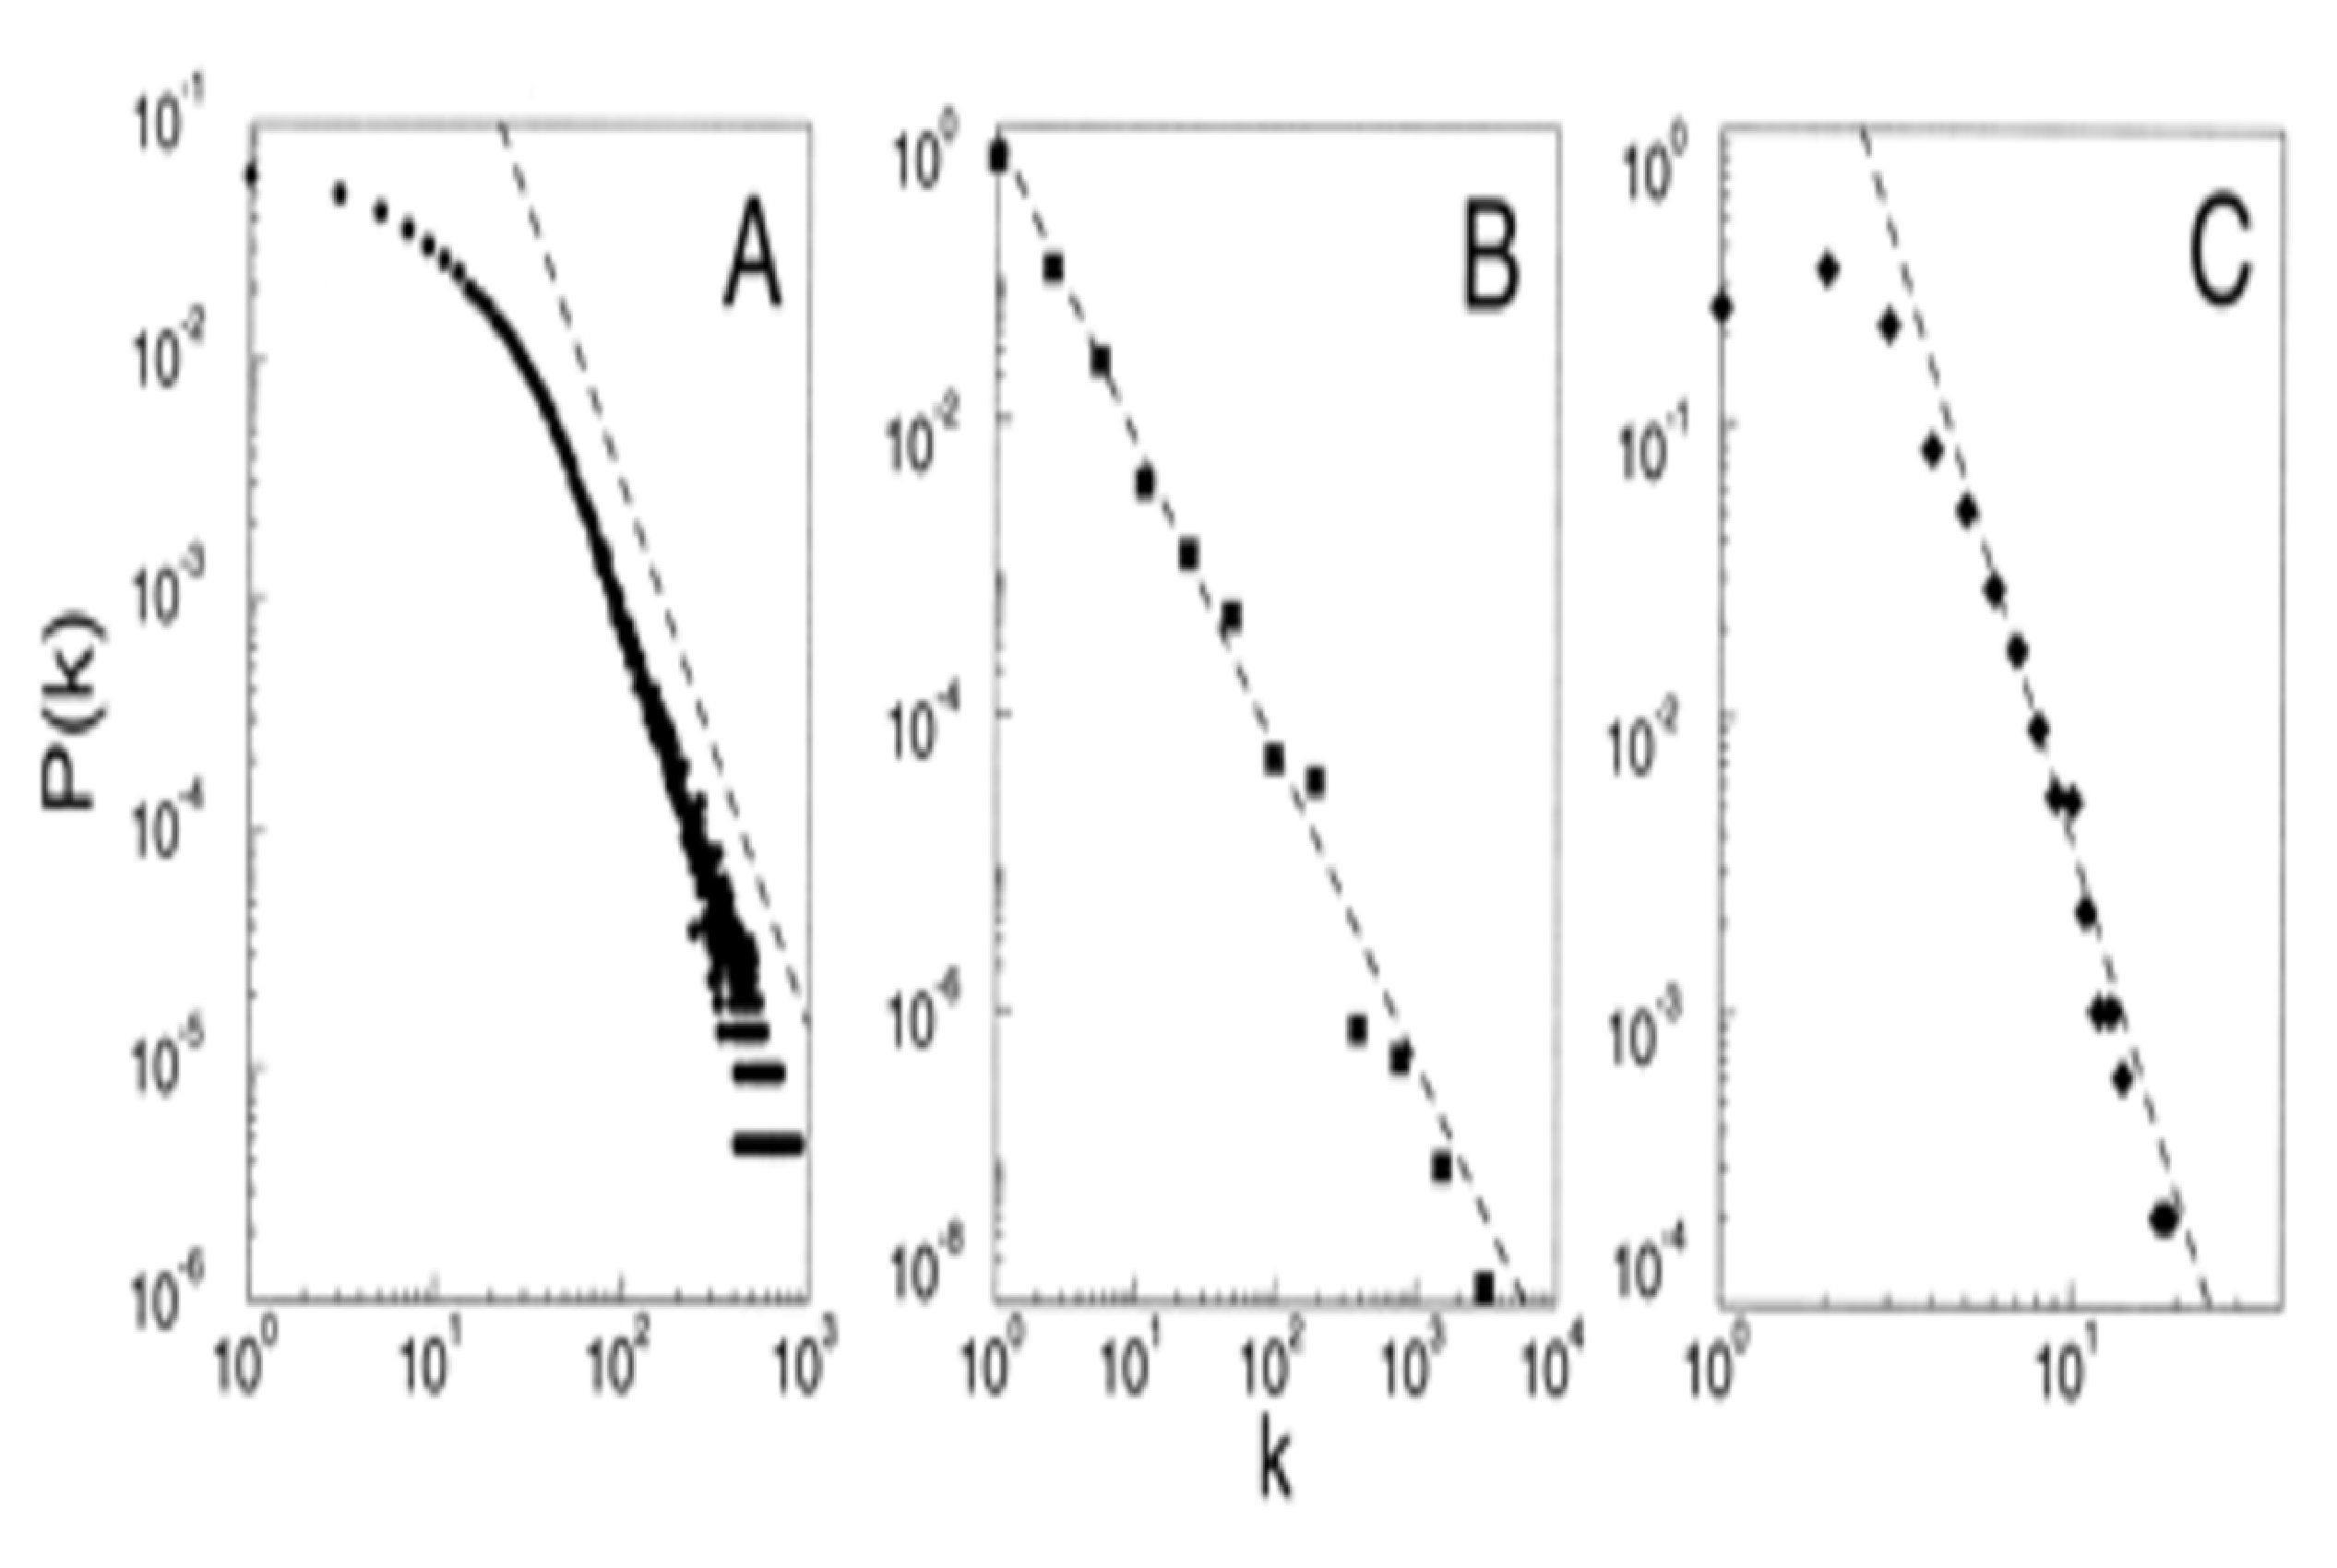
\includegraphics[scale=0.3]{./figures/scal-free-reels}
\caption{Quelques exemples des réseaux sans-échelle, (\textbf{A}) Graphe de collaboration d'acteur avec un nombre des nœuds
$n=212250$ et un degré moyen $\textless k\textgreater=28.78$, (\textbf{B}) WWW, $n=325729$, $\textless k\textgreater=5.46$,
(\textbf{C}) Données du réseau électrique, $n=4941$ et $\textless k\textgreater=2.69$. Les lignes pointillées ont des pentes
(\textbf{A}) $\gamma_{actor}=2.3$, (\textbf{B}) $\gamma_{www}=2.1$ et (\textbf{C}) $\gamma_{electrique}=4$.}

\label{scal-free-reels}
\end{figure}
Les distributions de la loi de puissance se produisent dans une gamme de réseaux extraordinairement diversifiée, tels que, les populations des  villes \cite{New2005,Aa-al2009}, la taille des tremblements de terre \cite{GuR1944}, des cratères de la lune  \cite{NeI1994}, la fréquence d'utilisation des mots dans n'importe quelle langue humaine \cite{Zipf1949,Estoup1916}, la  fréquence de l'apparition de noms personnels dans la plupart des cultures \cite{ZaM2001}, le nombre de documents scientifiques écrits \cite{LoW1926}, le nombre de citations reçues par les documents \cite{Price1965}, le nombre de visites sur les pages Web \cite{AdH2000}, les ventes de livres, les enregistrements musicaux et presque tous les autres produits de marque \cite{Cox-al1995}, le nombre d'espèces dans les genres biologiques \cite{WilY1922}, les revenus annuels des personnes \cite{Pareto1896}, les collecteurs de réseaux quantiques complexes \cite{BiR2015} et une foule d'autres réseaux suivent toutes des distributions de loi de puissances.\\

Mathématiquement, une quantité $x$ obéit à une loi de puissance s'elle est tirée d'une distribution de probabilité
\begin{equation}
 P(x)\propto x^{-\gamma}
\end{equation}
Avec $\gamma$ est un paramètre constant de la distribution connue sous le nom d'exposant, empiriquement cet exposant se situe
généralement dans l'intervalle $2<\gamma<3$, bien qu'il existe des exceptions occasionnelles.

\subsection{Structure communautaire}
La société offre une grande variété d'organisations de groupes possibles: les familles, les milieux de travail et d'amitié, les villages, les villes, les nations (voir un exemple Fig.~\ref{community-network}). La diffusion d'Internet a également conduit à la création de groupes virtuels directement sur le Web. Ces communautés se forment également dans de nombreux systèmes en réseau, de la biologie, de l'informatique, de l'ingénierie, de l'économie, de la politique, etc. Par exemple dans le graphe du World Wide Web les communautés peuvent correspondre à des groupes de pages portant sur les mêmes sujets ou des sujets connexes \cite{Dou-al2007,Flak-al2002}. Dans les réseaux d'interactions protéines-protéines, les communautés sont susceptibles de regrouper des protéines ayant la même fonction spécifique dans la cellule \cite{ChY2006,RivT2003}.\\

\begin{figure}[h!]
	\centering
	\includegraphics[scale=0.55]{./figures/community-network}
	\caption{Exemples d'un réseau communautaire, chaque couleur représente un groupe plus connecté par rapport au reste du réseau.}
	\label{community-network}
\end{figure}

Les communautés peuvent avoir des applications concrètes. Le Clustering des clients Web qui ont des intérêts similaires et qui sont géographiquement proches les uns des autres peut améliorer la performance des services fournis sur le WWW, en ce sens chaque groupe de clients pourrait être servi par un serveur miroir dédié \cite{KriW2000}.
Les réseaux auto-configurés formés par des nœuds de communication agissant dans la même région et changeant rapidement n'ont généralement pas de tables de routage centralisées qui spécifient comment les nœuds doivent communiquer entre eux.
Dans ce cas le regroupement des nœuds en clusters permet de générer des tables de routage compactes et rend le choix des chemins de communication plus efficace \cite{Steen2001}.\\
La détection communautaire est également importante pour d'autres raisons. L'identification des modules et de leurs limites permet une classification des nœuds, en fonction de leur position structurelle dans les modules. Donc, les nœuds avec une position centrale dans leurs grappes partagent un grand nombre de bords avec les autres partenaires du groupe, ce qui est une caractéristique importante de contrôle et de stabilité au sein du groupe, en outre, Les nœuds situés aux frontières entre les modules jouent un rôle important de médiation et mènent les relations et les échanges entre les différentes communautés \cite{Csermely2008}.

\section{Les modèles théoriques les plus connus} 

De façon générale on peut distinguer trois modèles des réseaux: aléatoire, de petit monde et le modèle sans-échelle. Ces modèles se caractérisent chacun par la manière dont les réseaux sont créés et par plusieurs statistiques résultantes, telles que la distribution des degrés, la longueur moyenne entre les paires de nœuds et le coefficient de Clustering.

   \subsection{Réseau aléatoire d'Erd\H{o}s-Rényi}
   
 Un réseau aléatoire est créé en spécifiant que chaque paire de nœuds est connecté par un lien avec une probabilité uniforme $p$. Ce type de réseaux a été étudié d'un point de vue mathématique pure par Erd\H{o}s et Rényi (ER) \cite{Erdos-Renyi1959,Erdos-Renyi1960,Erdos-Renyi1961}, il est souvent désigné par son nom mathématique $G(n,m)$, avec $n$ est le nombre de nœuds et $m$ le nombre de liens. 
 Dans la cas où $n$ est très grand, bon nombre de propriétés de l'ensemble des réseaux aléatoires ont été exprimées analytiquement de façon parfaite et élégante.\\
 Les graphes aléatoires ER sont les mieux étudiés parmi les modèles de graphes, leurs propriétés structurelles varient en fonction de $p$ montrant notamment un changement radical à une probabilité critique $p_c=\frac{1}{n}$,
 correspondant à un degré moyen critique $\textless k \textgreater_c=1$. Erdös et Rényi ont prouvé que:\\
 \begin{itemize}
  \item Si $p <p_c$, lorsque $n$ tend vers l'infini, le graphe n'a quasiment pas de composante de taille  
  supérieure à $(ln(n))$.
  \item Si $p=p_c$, la composante la plus importante a quasiment la taille de $n^{\frac{2}{3}}$.
  \item Si $p> p_c$, le graphe a une composante de taille de l'ordre de $n$ et aucune autre composante n'a de taille supérieure à $(ln(n))$.
 \end{itemize}
\begin{figure}[h!]
	\centering
	\includegraphics[width=12cm,height=9cm]{./figures/fig-ER-CG}
	\caption{Les simulations numériques du seuil de percolation dans le modèle ER en fonction du degré moyen, pour un réseau de taille $n=10^5$. On observe que le point où la fraction de la composante géante, $S$, émerge est à $\textless k\textgreater=1$ .}
	
	\label{percolation-graph}
\end{figure}

La transition au $p_c$ présente les caractéristiques typiques d'une transition de phase de deuxième ordre. En particulier, si on considère la taille de la composante la plus importante comme paramètre d'ordre, la transition tombe dans la même classe d'universalité que celle des transitions de percolation de champ moyen (voir Fig.~\ref{percolation-graph}). Erdös et Rényi ont étudié la distribution des degrés minimum et maximum dans le graphe aléatoire, mais la distribution des degrés complet a été obtenue plus tard par Bollobás \cite{Bollobas1998}. La probabilité qu'un nœud possédant le degré  $k$ est la distribution binomiale:
\begin{equation}
P(k)=C^k_{n-1}p^k(1-p)^{n-1-k}
\end{equation}
 Pour $n$ très grand, la répartition du degré est bien approchée par une distribution de Poisson:
 \begin{equation}
 P(k)=e^{-\textless k\textgreater}\dfrac{\textless k\textgreater^k}{k!}
 \label{ER}
 \end{equation}
\begin{figure}[h!]
	\centering
	\includegraphics[scale=1]{./figures/fig-ER-dist}
	\caption{Illustration de la distribution des degrés d'un réseau aléatoire ER de degré moyen égale $6$, les cercles représentent les simulations numériques et la ligne noire représente Eq.~\eqref{ER}.}
	
	\label{ER-distribution}
\end{figure} 

 Le coefficient de regroupement, $C$, est une quantité très simple à calculer pour le graphe aléatoire de Poisson, rappelons qu'il est défini comme la probabilité que deux voisins d'un nœud du réseau soient également voisins les uns des autres. Dans un graphe aléatoire, la probabilité que les deux nœuds soient voisins est égale à $p=\frac{\textless k\textgreater}{(n - 1)}$. Par conséquent:
 
 \begin{equation}
 C=\dfrac{\textless k\textgreater}{(n - 1)}
 \end{equation}
 
Cette valeur de Clustering qui tend vers $0$ quand $n$ tend vers l'infini est l'un des nombreux aspects dans lesquels le graphe aléatoire diffère fortement de la plupart des réseaux réels, dont beaucoup ont des coefficients de regroupement assez élevés.
 
 
 \subsection{Le modèle petit-monde de Watts-Strogatz}
 

   Le réseau aléatoire ER reproduit très bien l'observation concernant la longueur moyenne relativement petite des chemins, mais le coefficient de regroupement (Clustering) dans ce réseau est très faible par rapport à ceux observés dans les systèmes réels, et la distribution des degrés est déférente de celle du réseau réel. En 1998 Watts et Strogatz \cite{Watss-Strogatz1998} ont proposé un modèle qui reproduit deux propriétés parmi celles mentionnées précédemment de manière simple.\\
   Les modèles de petit-monde peuvent être construits sur des réseaux de n'importe quelle dimension ou topologie, mais le cas le mieux étudié est l'unidimensionnel. Soit $n$ le nombre de nœuds et $k$ un nombre pair, le modèle Watt-Strogatz commence par la construction suivante (voir Fig.\ref{SW1}): 
   \begin{itemize}
   	\item Placez tous les noeuds en cercle;
   	\item Connectez chaque nœud à ses premiers $k$ voisins les plus proches;
   	\item  Avec une probabilité $p$ en prenant chaque lien du réseau et on le reconnecte.
   \end{itemize}
   \begin{figure}[h!]
   	\centering
   	\includegraphics[scale=0.6]{./figures/SW1}
   	\caption{Représentation schématique de l'évolution du processus de "reconnexion" dans le modèle Watts-Strogatz.}  	
   	\label{SW1}
   \end{figure}

Ce modèle peut être justifié en disant que la plupart des gens sont amis avec leurs voisins immédiats,  par exemple les voisins de la même rue ou des collègues du même bureau. D'autre part, beaucoup des gens ont quelques amis qui se vivent loin. Les propriétés structurelles du modèle sont quantifiées par la longueur de chemin caractéristique $L(p)$ et le coefficient de regroupement $C(p)$ en tant que fonctions de la probabilité de reconnecter $p$. La longueur de chemin caractéristique $L$ est définie comme la valeur moyenne de nombre d'arêtes dans le chemin le plus court entre deux nœuds.\\
Nous savons que le réseau ordinaire à $p=0$ est un grand monde en grappe, où $L$ se développe linéairement avec $n$, tandis que le graphe aléatoire à $p=1$ est un petit monde faiblement regroupé où $L$ ne se développe que logarithmiquement avec $n$. 
\begin{figure}[h!]
	\centering
	\includegraphics[scale=0.75]{./figures/SW2}
	\caption{Représentation de la variation de la longueur moyenne du chemin $L(p)$ et du coefficient de regroupement $C(p)$ avec la modification de la probabilité de reconnexion $p$ dans le modèle Watts-Strogatz.}  	
	\label{SW2}
\end{figure}


Selon Fig.~\ref{SW2} on voit que l'introduction de quelques bords à longue distance entraîne une baisse immédiate de $L(p)$, par contre $C(p)$ reste pratiquement inchangé pour les petites $p$ même si $L(p)$ chute rapidement. L'implication importante est que, au niveau local, la mise à l'échelle du petit monde de la distance géodésique moyenne entre les nœuds peut se produire pour les mêmes valeurs de $p$ auxquelles le coefficient de regroupement local du réseau est significativement important.\\
Le plus court chemin moyen a été montré comme \cite{Barthelemy-Amaral1999,Newman-al2000}
\begin{equation}
  L\sim \frac{n}{k}f(x),
\end{equation}
avec $x$ le nombre moyen des bords qui se reconnectent dans le réseau et $f(x)$  une fonction universelle qui a les formes asymptotiques suivantes:
\begin{align}
f(x)&\sim
\begin{cases}
\dfrac{1}{4} & \text{si } x \gg1\\
\\
\dfrac{\log\mathrm{2x}}{\mathrm{4x}}& \text{si } x \ll1.
\end{cases}
\end{align}

   Le coefficient de regroupement C est défini par Eq.~\eqref{Clustering}, que nous reproduisons ici:
 \begin{equation}
 C=\frac{3\times\text{(Nombre de triangles)}}{\text{(Nombre de triples connectés)}}.
 \end{equation}  
Pour évaluer $C$, nous devons calculer le nombre de triangles et les triplets connectés dans le réseau, alors on va trouver la valeur moyenne de $C$ comme la suite \cite{Newman2010-558}:
\begin{equation}
C=\frac{3(k-1)}{4(k-1)+8kp+4kp^2}.
\end{equation}  

En ce qui concerne la répartition de degré, lorsque $p=0$ est une fonction delta positionnée à $k$, alors que pour $p=1$ elle est similaire à celle d'un réseau ER. Pour les valeurs intermédiaires de $p$, la répartition du degré est donnée par \cite{Barrat-Weigt2000}:
\begin{equation}
P(k)=\sum_{i=0}^{\text{min}(k-m,m)}C_i^m\frac{(pm)^{k-m-i}}{(k-m-i)}e^{pm}.
\end{equation} 

   \subsection{Le modèle sans-échelle de Barabási-Albert}
   
Une caractéristique commune entre le graphe aléatoire ER et les modèles de petit-monde de WS est que la distribution des degrés du réseau est homogène, avec un pic à une valeur moyenne et une décroissance exponentielle, de tels réseaux s'appellent des réseaux exponentiels. Les inconvénients de ces deux modèles précédents est qu'ils ne tiennent pas compte de deux attributs importants de la plupart des réseaux réels.  Premièrement, les réseaux réels sont ouverts et ils sont dynamiquement formés par l'ajout continu de nouveaux nœuds au réseau, par exemple, la WWW génère continuellement de nouvelles pages Web et la littérature de recherche se développe constamment car les nouveaux articles sont en cours de publication. Deuxièmement, le graphique aléatoire ER et le modèle de petit-monde prennent des probabilités uniformes lors de la création de nouvelles arêtes, mais ce n'est pas réaliste non plus.

Une découverte relativement récente et importante dans le domaine des réseaux complexes est l'observation qu'un certain nombre de réseaux complexes à grande échelle, y compris Internet, WWW et les réseaux métaboliques, sont sans échelle et leurs distributions de connectivité ont une forme de puissance (voir Fig.~\ref{scal-free-reels}).\\
Nous parlons alors ici d'une classe de modèles dont l'objectif principal est de reproduire les processus de croissance qui se déroulent dans des réseaux réels. Nous nous concentrons principalement sur le modèle de croissance du réseau proposé par Barabási et Albert en 1999 \cite{BA1999}, ce modèle repose sur deux hypothèses simples concernant l'évolution du réseau:
\begin{itemize}
	\item \textbf{Croissance}: De nouveaux nœuds sont ajoutés au réseau, chaque nouveau nœud étant connecté à $m$ des nœuds existants.
	\item \textbf{Attachement préférentielle}: Chaque nouveau nœud est connecté aux nœuds existants avec une probabilité proportionnelle à son degré.
\end{itemize}
De manière plus détaillée, considérons un réseau évoluant dans le temps, $t$, où, à chaque fois, un nouveau nœud est ajouté au réseau et connecté à $m$ des nœuds existants, où la probabilité de se connecter à un nœud existant,  $i$, $\Pi(i)$ est donné par:
\begin{equation}
\Pi(i)=\dfrac{k_i}{\sum_jk_j}.
\end{equation}
Le nombre de nœuds initial à l'instant $t=0$ est généralement supposé être connecté et doit être supérieur à $m$, mais les détails de sa structure n'ont qu'un faible effet sur le résultat final.\\

Il existe plusieurs méthodes pour analyser les résultats du modèle Barabási-Albert.
La méthode la plus simple est une analyse de champ moyen décrite initialement dans \cite{BA1999}.
D'autres méthodes plus rigoureuse d'analyse de ce modèle utilisant des outils de la physique statistique comprennent l'approche de l'équation maîtresse \cite{Dorogovtsev-al2000} et l'approche de l'équation du taux \cite{Krapivsky-al2000}. La distribution des degrés trouvée est décrite par une loi de puissance avec l'exposant $-3$, c'est-à-dire que la probabilité de trouver un nœud avec le degré $k$ est proportionnelle à $k^{-3}$ (voir Fig.~\ref{BA-distribution}). plus précisément l'expression exacte de $P(k)$ est:
\begin{equation}
 P(k)=\dfrac{2m(m+1)}{k(k+1)(k+2)}.
\label{pk-1}
\end{equation}

L'Eq.~\eqref{pk-1} a d'abord été dérivée par Krapivsky et al. \cite{Krapivsky-al2000} et de manière indépendante par Dorogovtsev et al. \cite{Dorogovtsev-al2000-2}. Un traitement plus détaillé a ensuite été donné par Bollobas et al. \cite{Bollobas-Riordan2002}, qui clarifie précisément le domaine de validité de la solution et les écarts éventuels par rapport à la valeur attendue de  $P(k)$ .

\begin{figure}[h!]
	\centering
	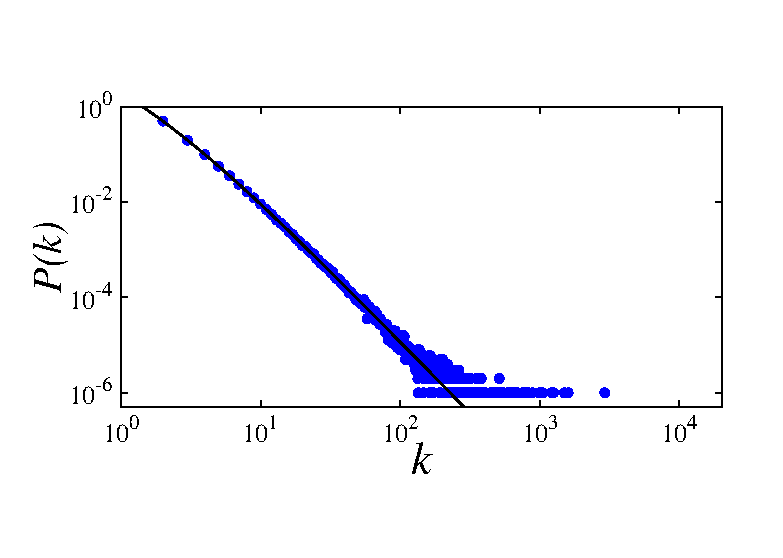
\includegraphics[scale=1]{./figures/fig-barabasi}
	\caption{La distribution des degrés du réseau BA en échelle logarithmique, où les cercles sont les simulations numériques et la ligne continue représente la formule théorique, Eq.~\eqref{pk-1}. La taille du réseau est $\mathrm{n}=10^{6}$ et $\mathrm{m}=2$ .}	
	\label{BA-distribution}
\end{figure} 

La distance moyenne dans le modèle BA est plus petite que dans le graphe aléatoire ER. Les résultats analytiques prédisent une correction de double logarithmique qui diminue la dépendance logarithmique $ L\sim\frac{\log \mathrm{N}}{\log\log\mathrm{N} }$ \cite{Bollobas-Riordan2002}. Le coefficient de regroupement décroît avec la taille du système comme $C\sim N^{-0,75}$. Il s'agit d'une décroissance plus lente que celle observée pour les graphes aléatoires, $C\sim N^{-1}$, mais le comportement reste différent par rapport aux modèles du petit monde, où $C$ est une constante indépendante de la taille du réseau $\mathrm{N}$.